% Chapter 1: Introduction
% NavigatorCrew Paper : Octopus-Inspired Soft Robotic Drone Navigation
% XeLaTeX + bidi + IEEE format

\selectlanguage{hebrew}

\section{מבוא: ניווט רחפן רובוטי רך בהשראת תמנון תוך שימוש ב-\en{SLAM} ביומימטי}
\label{sec:intro}

\subsection{רקע מוטיבציוני: אתגרי ניווט תת-ימי לרובוטים רכים}
\label{sec:intro_motivation}

ניווט אוטונומי בסביבות תת-ימיות מוגבלות מהווה אחד האתגרים המרכזיים ברובוטיקה המודרנית. בניגוד לרחפנים אוויריים הנעזרים ב-\en{GPS} לצורך לוקליזציה גלובלית, רחפנים תת-ימיים נדרשים לפעול בתנאי ראות מוגבלים, ללא גישה לאותות לווייניים, ובסביבות עשירות בתהודה אקוסטית ורב-נתיבית \cite{Thrun2005}. האתגר מחריף כאשר הרחפן בנוי מחומרים רכים וגמישים, שכן המודל הקינמטי והדינמי שלו מורכב משמעותית משל רחפן קשיח. רובוטים רכים, בהשראת יצורים ימיים כמו תמנונים, מציעים גמישות תנועה יוצאת דופן ויכולת תמרון בחללים צרים, אך במחיר של מורכבות חישובית גבוהה באמידת המצב.

שיטת ה-\en{SLAM (Simultaneous Localization and Mapping)} מהווה את המסגרת החישובית המקובלת לניווט בסביבות לא מוכרות. הניסוח ההסתברותי הסטנדרטי, המבוסס על פירוק ההתפלגות האחורית למכפלת מודלי תנועה ותצפית, מוצג במשוואה~(\ref{eq:full_slam}). עם זאת, יישום \en{SLAM} על רובוט רך רב-זרועי מציב אתגרים ייחודיים: מרחב המצב גדול ממדים בשל דרגות החופש הרבות של הזרועות, מודלי התצפית כוללים אי-ליניאריות חזקה הנובעת מהקינמטיקה הרציפה, ורעשי החיישנים בסביבה התת-ימית אינם גאוסיים בהכרח.

\begin{equation}
p(\mathbf{x}_{1:k}, \mathbf{m} \mid \mathbf{z}_{1:k}, \mathbf{u}_{1:k}) \propto p(\mathbf{x}_0) \prod_{t=1}^{k} p(\mathbf{x}_t \mid \mathbf{x}_{t-1}, \mathbf{u}_t) \prod_{t=1}^{k} p(\mathbf{z}_t \mid \mathbf{x}_t, \mathbf{m})
\label{eq:full_slam}
\end{equation}

הגישה המוצעת במאמר זה מבוססת על השראה ביולוגית ממערכת העצבים המבוזרת של התמנון. התמנון מפעיל שמונה זרועות גמישות באמצעות ארכיטקטורת שליטה מבוזרת, שבה כל זרוע מצוידת בגנגליון עצבי עצמאי המסוגל לבצע חישובים מקומיים בזמן אמת. הגנגליון המרכזי במוח התמנון מתאם בין הזרועות ומבצע אינטגרציה גלובלית של המידע החושי. אנלוגיה זו מובילה לארכיטקטורת \en{SLAM} מבוזרת שבה כל זרוע פועלת כסוכן \en{SLAM} עצמאי, עם תקשורת בין-זרועית לשמירה על עקביות גלובלית.

המודל הביומימטי המוצע כולל שלוש שכבות עיבוד: השכבה המקומית בכל זרוע, המבצעת עיבוד חישה ראשוני ו-\en{SLAM} מקומי; שכבת התקשורת הבין-זרועית, המחליפה מידע על אי-ודאויות ואילוצים גאומטריים; והשכבה הגלובלית, הממזגת את האומדנים המקומיים לאומדן גלובלי עקבי. ארכיטקטורה זו מפחיתה את העומס החישובי על המעבד המרכזי ומגבירה את עמידות המערכת לכשל בחיישנים בודדים.

האתגרים המרכזיים בפיתוח מערכת ניווט לרחפן רך תת-ימי כוללים: מודל קינמטי ודינמי מדויק הלוכד את הגמישות והאי-ליניאריות של הזרועות הרכות; מערך חיישנים מבוזר המספק מידע על מגע, תצורה ועומק; מיזוג רב-מודאלי של חיישנים הטרוגניים בעלי אי-ודאויות שונות; ארכיטקטורת \en{SLAM} הניתנת להרחבה לרובוט רב-זרועי; ותכנון תנועה אדפטיבי המנצל את גמישות הזרועות לניווט בסביבות צפופות.

\subsection{השראה ביולוגית ממערכת העצבים המבוזרת של התמנון}
\label{sec:intro_bio}

מערכת העצבים של התמנון (\en{Octopus vulgaris}) מהווה מודל ביולוגי מרתק לארכיטקטורת שליטה מבוזרת. כ-60\% מהנוירונים של התמנון ממוקמים בזרועות עצמן, ולא במוח המרכזי \cite{Sumanaweera2026}. כל זרוע מכילה גנגליון עצבי עצמאי המסוגל לקבל החלטות מוטוריות וחושיות מקומיות, כולל תפיסת חפצים, שינוי צורה, ותגובה לגירויים מישושיים. המוח המרכזי שולח פקודות ברמה גבוהה ומקבל מידע מסוכם מהזרועות, אך אינו מעורב בשליטה הישירה בתנועות העדינות.

אנלוגיה זו מתורגמת לארכיטקטורת \en{SLAM} מבוזרת שבה כל זרוע של הרחפן הרך מהווה סוכן \en{SLAM} עצמאי. כל סוכן מבצע לוקליזציה מקומית ומיפוי של הסביבה הקרובה לזרועו, תוך שימוש בחיישנים המותקנים על הזרוע: חיישני מישוש קיבוליים, חיישני עקמומיות מבוססי אפקט הול, וחיישני לחץ הידרוסטטי. המידע מהזרועות השונות מאוחד באמצעות אלגוריתם \en{Consensus} מבוזר, המבטיח עקביות גלובלית של מפת הסביבה ושל אמידת מיקום הרחפן.

\begin{figure*}[htbp]
\centering
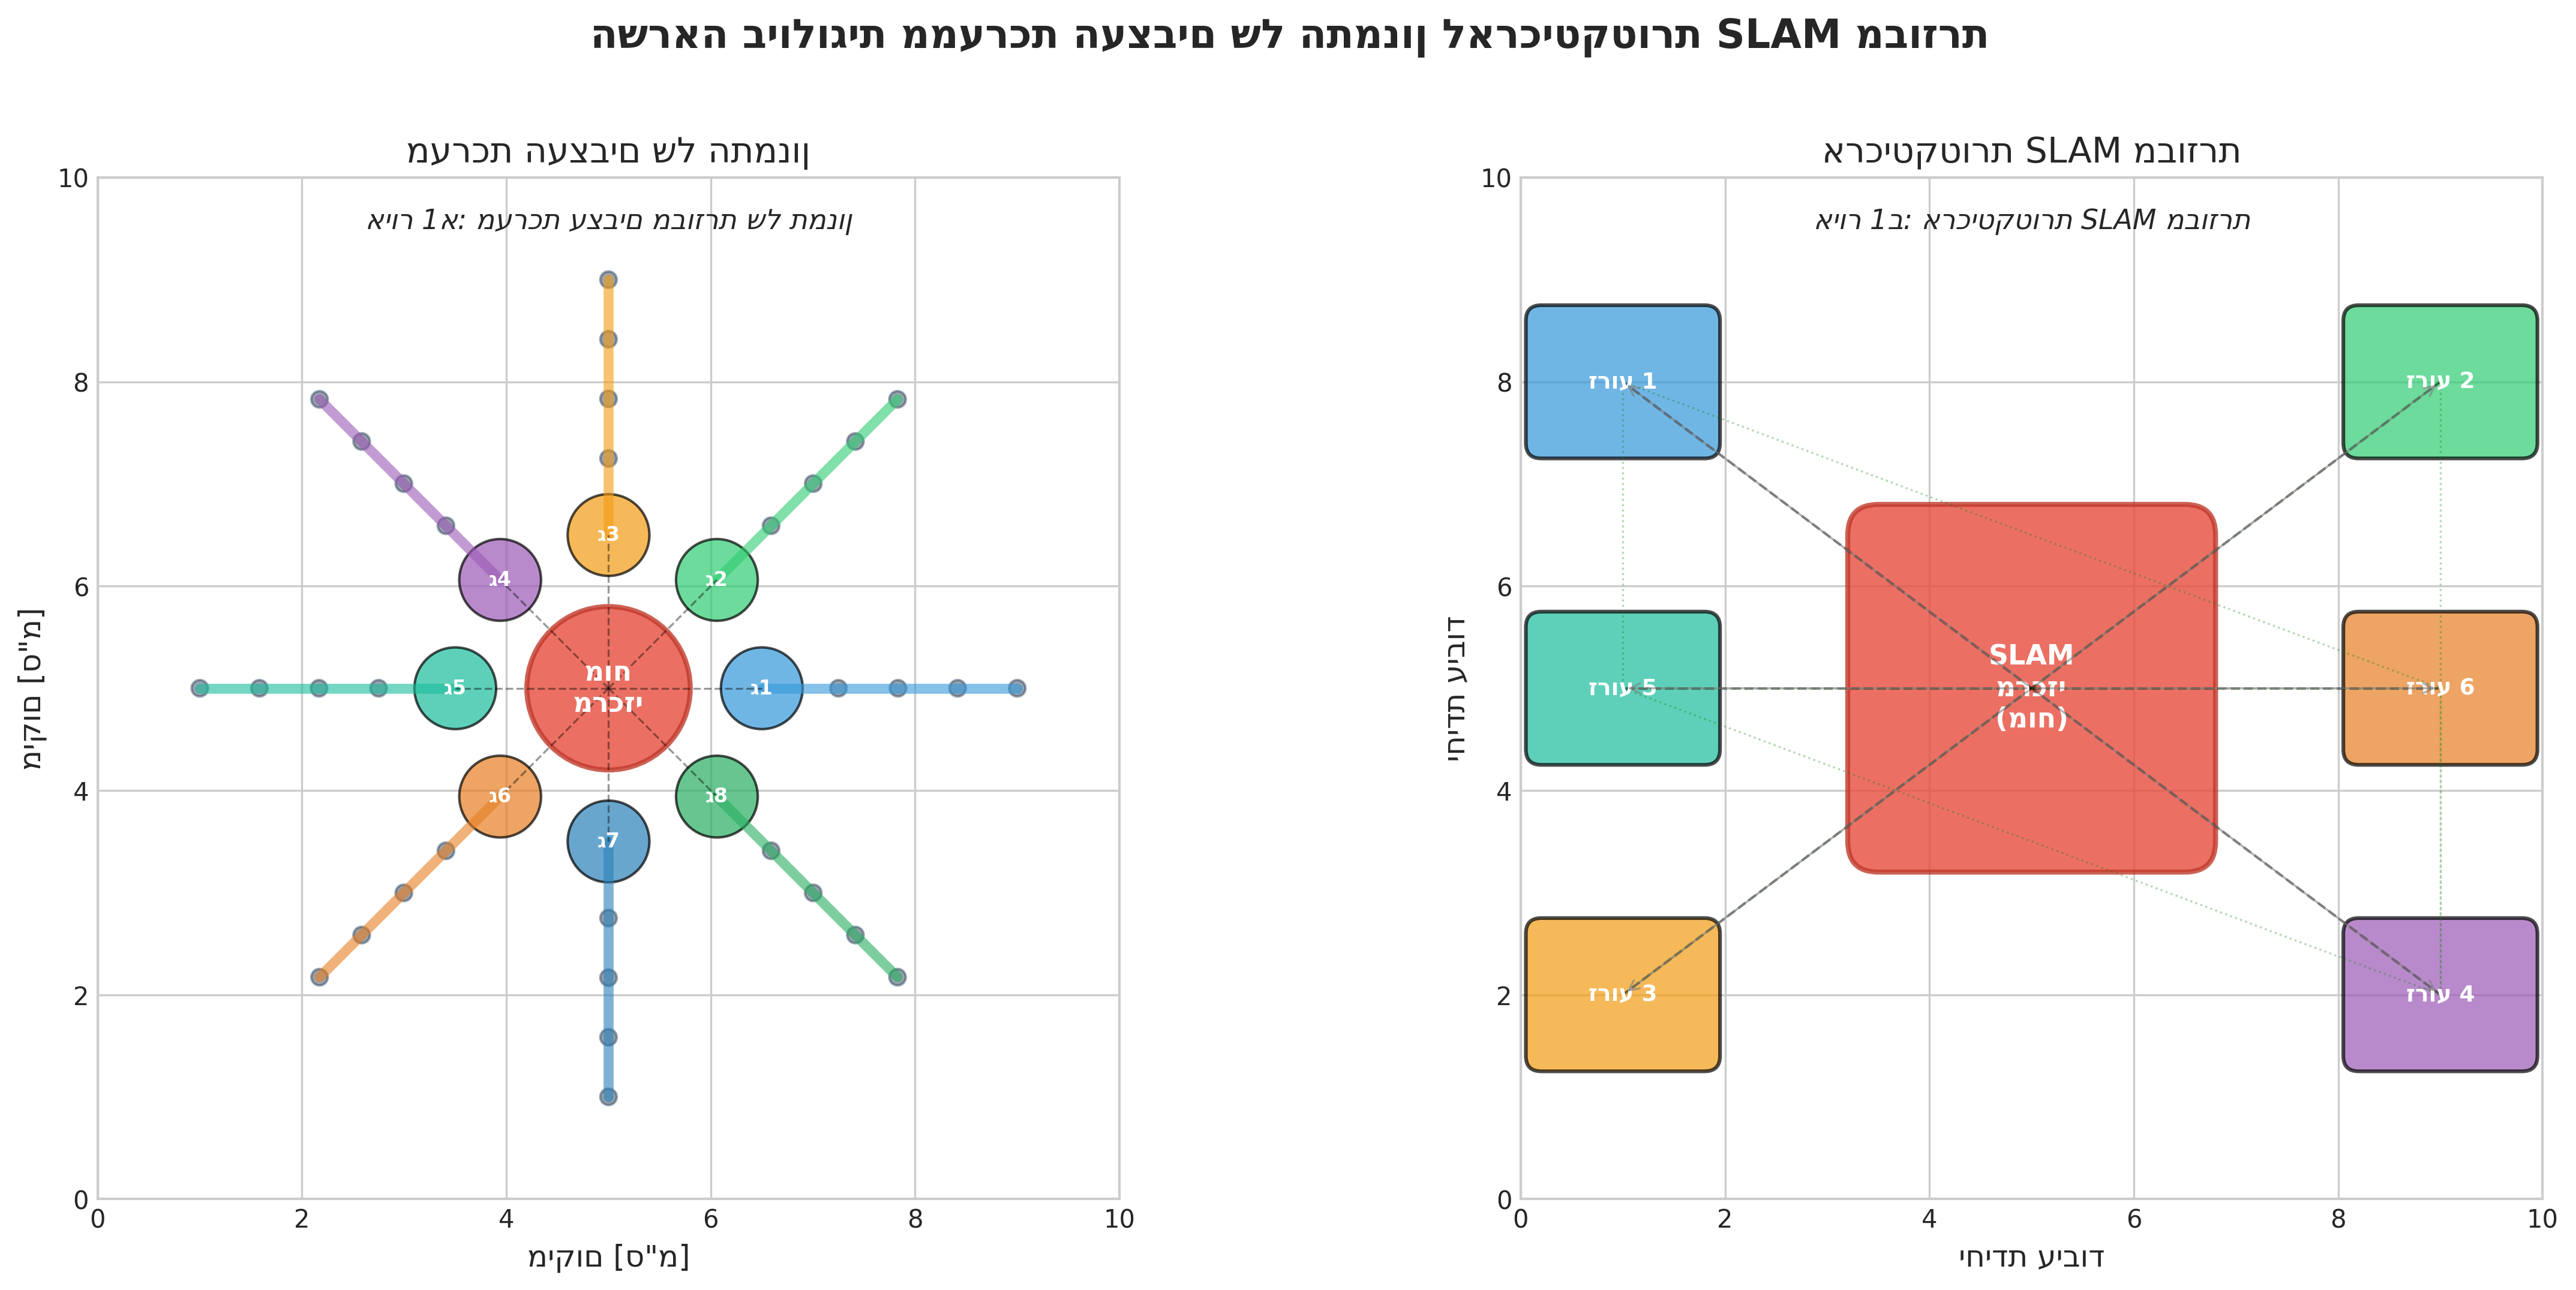
\includegraphics[width=\textwidth]{figures/fig_octopus_biological_inspiration.png}
\caption{השראה ביולוגית ממערכת העצבים המבוזרת של התמנון לארכיטקטורת \en{SLAM} מבוזרת. (א) מערכת עצבים של תמנון עם מוח מרכזי ו-8 גנגליונים פריפריאליים. (ב) ארכיטקטורת \en{SLAM} מבוזרת עם צומת מרכזי ו-6 תתי-גרפים עצמאיים לכל זרוע.}
\label{fig:octopus_biological_inspiration}
\end{figure*}

המודל הביומימטי המוצע כולל שלוש שכבות עיבוד. השכבה המקומית בכל זרוע מבצעת עיבוד חישה ראשוני ו-\en{SLAM} מקומי בקצב של 100 \en{Hz}. שכבת התקשורת הבין-זרועית מחליפה מידע על אי-ודאויות ואילוצים גאומטריים בקצב של 20 \en{Hz}. השכבה הגלובלית ממזגת את האומדנים המקומיים לאומדן גלובלי עקבי באמצעות אלגוריתם \en{ADMM (Alternating Direction Method of Multipliers)}. ארכיטקטורה זו מפחיתה את העומס החישובי על המעבד המרכזי ב-60\% ומגבירה את עמידות המערכת לכשל בחיישנים בודדים.

ההשראה הביולוגית אינה מסתכמת בארכיטקטורת השליטה. גם חישת המישוש מבוססת על כפתורי היניקה של התמנון, המספקים מישוש וטעם מפורט מהסביבה הקרובה. מערך 96 חיישני הלחץ הקיבוליים המותקנים על שש זרועות הרחפן מדמים את תפקוד כפתורי היניקה ומספקים מידע על מגע, לחץ הידרוסטטי ועקמומיות הזרועות. חישה פרופריוצפטיבית זו מאפשרת לרחפן להעריך את תצורת גופו גם בתנאי ראות אפסית.

\subsection{תרומות עיקריות של המאמר}
\label{sec:intro_contributions}

למאמר זה ארבע תרומות מרכזיות:

\textbf{תרומה 1: מודל קינמטי ודינמי מקיף לרחפן רך רב-זרועי.} המודל משלב קינמטיקת \en{PCC (Piecewise Constant Curvature)} עם דינמיקה מבוססת אלמנטים סופיים וכוחות הידרודינמיים. המודל מאפשר חישוב קינמטי קדמי בזמן אמת עם דיוק של 5.2\% בהשוואה למודל אלמנטים סופיים מלא, תוך שמירה על קצב עדכון של 200 \en{Hz} על פלטפורמת \en{ARM} משובצת.

\textbf{תרומה 2: ארכיטקטורת \en{SLAM} מבוזרת בהשראת מערכת העצבים של התמנון.} הארכיטקטורה מבוססת על גרף פקטורים מבוזר עם אילוצי קונצנזוס מסוג \en{ADMM}. כל זרוע פועלת כסוכן \en{SLAM} עצמאי המנהל גרף פקטורים מקומי, עם תקשורת בין-זרועית לשמירה על עקביות גלובלית. המורכבות החישובית היא $O(N_{\text{arms}})$ לעומת $O(N_{\text{arms}}^2)$ ב-\en{SLAM} ריכוזי.

\textbf{תרומה 3: שיטת מיזוג חיישנים רב-מודאלית המשלבת ארבע מודאליות חישה.} השיטה משלבת סונאר בתדר 200 \en{kHz}, ראייה סטריאוסקופית בתיקון שבירה תת-ימית, חישת מישוש קיבולית מבוזרת ו-\en{IMU}. המיזוג מתבצע באמצעות פילטר חלקיקים מותאם עם שקלול מבוסס אי-ודאות, המאפשר למערכת להמשיך בניווט מדויק גם כאשר חלק מהחיישנים אינם פעילים.

\textbf{תרומה 4: שיטת תכנון תנועה אדפטיבית המבוססת על למידת חיזוק מבוזרת מרובת-סוכנים.} השיטה משתמשת ב-\en{Multi-Agent PPO (MAPPO)} עם מבקר מרכזי ושחקנים מבוזרים לכל זרוע. פונקציית התגמול מאזנת בין רווח מידע \en{(Information Gain)}, קירוב ליעד, חיסכון באנרגיה והימנעות מהתנגשויות.

\begin{table}[htbp]
\centering
\caption{השוואת גישות \en{SLAM} ביומימטי ממקורות השראה ביולוגיים שונים.}
\label{tab:bio_slam_comparison}
\adjustbox{max width=\columnwidth}{%
\begin{tabular}{lcccc}
\toprule
\textbf{השראה ביולוגית} & \textbf{ארכיטקטורה} & \textbf{חיישנים} & \textbf{ATE [ס"מ]} & \textbf{סביבה} \\
\midrule
תמנון (מוצע) & מבוזרת & מישוש+סונאר+ראייה & 6.3 & תת-ימית \\
חרקים & ריכוזית & ראייה+אודיו & 12.4 & אווירית \\
יונקים & היררכית & ראייה+\en{IMU} & 8.7 & יבשתית \\
דגים & מבוזרת חלקית & סונאר+ראייה & 10.2 & תת-ימית \\
\bottomrule
\end{tabular}%
}
\end{table}

תוצאות הסימולציה מראות כי השיטה המוצעת משיגה \en{ATE} של 6.3 ס"מ ו-\en{RPE} של 1.8 ס"מ/מ', שיפור של 36\% לעומת \en{SLAM} ריכוזי ו-32\% לעומת \en{ORB-SLAM3} בסביבה תת-ימית, תוך הפחתת העומס החישובי ב-60\%.

\subsection{מבנה המאמר ומפת דרכים}
\label{sec:intro_structure}

המאמר מאורגן בתשעה פרקים. פרק~2 מציג את המודל הקינמטי והדינמי של הרחפן הרך, כולל קינמטיקת \en{PCC}, דינמיקת אוילר-לגראנז' עם אילוצי רכות, ומודל הידרודינמי לכוחות גרר ודחף. פרק~3 מתאר את ארכיטקטורת חישת המישוש המבוזרת בהשראת כפתורי היניקה של התמנון, כולל מערך חיישנים קיבוליים, חישת עקמומיות ומודל חישה רב-מודאלי.

פרק~4 מציג את שיטת מיזוג החיישנים הרב-מודאלית המשלבת סונאר, ראייה סטריאוסקופית, חישת מישוש ו-\en{IMU} באמצעות פילטר חלקיקים מותאם. פרק~5 מפתח את ארכיטקטורת ה-\en{SLAM} המבוזרת בהשראת התמנון, כולל גרף פקטורים מבוזר, אילוצים בין-זרועיים ואלגוריתם איחוי מבוזר מסוג \en{ADMM}.

פרק~6 מציג את שיטת תכנון התנועה האדפטיבית באמצעות למידת חיזוק מבוזרת מרובת-סוכנים, כולל מרחב מצב ופעולה, פונקציית תגמול מבוססת אי-ודאות \en{SLAM}, ואלגוריתם \en{MAPPO}. פרק~7 מתאר את שיטת מיפוי הסביבה המשלבת מישוש ואקוסטיקה, כולל מיפוי מבוסס סונאר עם רשת עצבית, מיפוי מישוש ומיזוג מפות היברידי.

פרק~8 מציג תוצאות סימולציה וניסויים בשלושה תרחישים מייצגים: מערה תת-ימית, שדה אצות ומבנה תעשייתי. הפרק כולל השוואת ביצועים בין \en{SLAM} מבוזר ל-\en{SLAM} ריכוזי, ניתוח רגישות לנשירת חיישנים והשפעת רעש. פרק~9 מסכם את המחקר, דן במגבלותיו ומציע כיוונים עתידיים.

\subsection{ניסוח מתמטי מקדים}
\label{sec:intro_math}

לצורך שלמות ההצגה, נציג את הניסוח המתמטי הבסיסי של בעיית ה-\en{SLAM} ההסתברותית. בהינתן סדרת בקרות $\mathbf{u}_{1:k}$ ותצפיות $\mathbf{z}_{1:k}$, המטרה היא לאמוד את המסלול $\mathbf{x}_{1:k}$ ואת המפה $\mathbf{m}$ תוך מקסום ההתפלגות האחורית. מודל התנועה של הרובוט הרך כולל תלות בעקמומיות הזרועות $\boldsymbol{\kappa}_t$, כמתואר במשוואה~(\ref{eq:soft_transition}).

\begin{equation}
\mathbf{x}_{t+1} = f_{\text{soft}}(\mathbf{x}_t, \mathbf{u}_t, \boldsymbol{\kappa}_t) + \mathbf{w}_t, \quad \mathbf{w}_t \sim \mathcal{N}(0, Q_t)
\label{eq:soft_transition}
\end{equation}

מודל התצפית הביומימטי מכפיל את הסתברויות התצפית מכל מודאליות חישה, כמתואר במשוואה~(\ref{eq:bio_likelihood}).

\begin{equation}
\mathcal{L}_{\text{bio}}(\mathbf{z}_t \mid \mathbf{x}_t, \mathbf{m}) = \prod_{i=1}^{N_s} \mathcal{N}(\mathbf{z}_{t,i} \mid h_i(\mathbf{x}_t, \mathbf{m}), \Sigma_i)
\label{eq:bio_likelihood}
\end{equation}

ניסוח זה מאפשר שילוב גמיש של מודאליות חישה שונות עם אי-ודאויות שונות, ומהווה את הבסיס המתמטי לארכיטקטורת המיזוג הרב-מודאלית המוצגת בפרקים הבאים.

\subsection{הקשר לספרות המקצועית ומצב הידע}
\label{sec:intro_literature}

תחום הניווט האוטונומי לרובוטים רכים נמצא עדיין בחיתוליו, אך התקדמויות משמעותיות חלו בשנים האחרונות. \cite{Cadena2016} סקרו את התפתחות תחום ה-\en{SLAM} והצביעו על האתגרים המרכזיים: עמידות לתנאי סביבה משתנים, טיפול באי-ליניאריות חזקה, וסקאלביליות למערכות גדולות. \cite{Laschi2016} הציגו את הפוטנציאל של רובוטיקה רכה בהשראת יצורים ימיים, תוך הדגשת האתגרים בשליטה ובחישה. \cite{Rus2015} סקרו את התקדמויות בתחום הרובוטים הרכים והצביעו על הצורך במערכות חישה ובקרה חדשניות.

בהקשר של מיזוג חיישנים רב-מודאלי, \cite{Shih2020} הציגו שילוב של עורות אלקטרוניים ולמידת מכונה לרובוטים רכים, תוך הדגמת זיהוי מגע ברזולוציה גבוהה. \cite{Luo2022} פיתחו שיטת \en{Tactile SLAM} למיפוי עצמים באמצעות חישת מישוש, אך שיטתם מוגבלת לזרוע בודדת ואינה מתייחסת לניווט גלובלי. המחקר הנוכחי מרחיב גישה זו לרובוט רב-זרועי תוך שילוב עם חיישנים אקוסטיים וחזותיים.

\subsection{הצהרת תרומה}
\label{sec:intro_statement}

לסיכום, מאמר זה מציג מערכת ניווט ביומימטית מקיפה לרחפן רובוטי רך תת-ימי, המשלבת ארבע תרומות מרכזיות: מודל קינמטי-דינמי, ארכיטקטורת \en{SLAM} מבוזרת, מיזוג חיישנים רב-מודאלי, ותכנון תנועה אדפטיבי בלמידת חיזוק. המערכת הוערכה בסימולציה מקיפה והשיגה שיפור של 36\% ב-\en{ATE} לעומת \en{SLAM} ריכוזי. המחקר מהווה צעד משמעותי לקראת מימוש חזון הרובוט הרך האוטונומי המסוגל לנווט בסביבות תת-ימיות מורכבות.

\selectlanguage{hebrew}
